
\chapter{Anleitung zur Benutzung des Java-Interpolators}\label{Handbuch}
\minitoc
\newpage
\section{Einleitung}
Im Rahmen dieser Diplomarbeit entstand neben einer neuen Algebra f"ur SECONDO, auch eine Java-Anwendung, die die selbe Arbeitsweise wie die Algebra aufweist. Die Benutzung dieses Tools wird im Folgenden erl"autert.

Das Tool dient in erster Line dem besseren Verst"andnis, wie die Algebra funktioniert. Ein Import oder Export mit SECONDO ist nicht m"oglich.

\section{Starten des Tools}
Das Tool ist in Java geschrieben, und liegt als Jar-Datei vor. Um das Programm ausf"uhren zu k"onnen, muss deshalb eine Java Laufzeitumgebung ab Version~1.4 vorhanden sein. Ist dies der Fall, so l"asst sich das Programm mittels \begin{verbatim}
java -jar MCInterpolator.jar
\end{verbatim}  starten.

Es erscheint der Startbildschirm Abbildung~\vref{fig:start}.

Dieser l"asst sich in vier Bereiche unterteilen:
\begin{itemize}
\item Eine Toolbar, die den VRML-Export Button und den Zeit-Einsteller beinhaltet. 
\item Die Zeichen-Toolbar, wozu sich nähere Informationen im Kapitel ,,Zeichnen einer Region`` finden.
\item Der Zeichenbereich, wo man neue Regionen zeichnen kann und importierte Regions betrachtet.
\item Die Umschaltfl"achen,  mit denen zwischen den verschiedenen Werkzeugen gewechselt werden kann. Nach dem Starten findet sich hier neben der Zeichenf"ache nur Konfigurationsschaltfl"ache, die im Kapitel ,,Konfigurieren des Matchings`` n"aher beschrieben werden. Schlie"st man die Zeichnung von zwei Regions ab, tauchen weitere Schaltfl"achen auf, die im Kapitel ,,Die verschiedenen Ergebnisansichten`` erl"autert werden.
\end{itemize} 

\begin{figure}
   \centering
   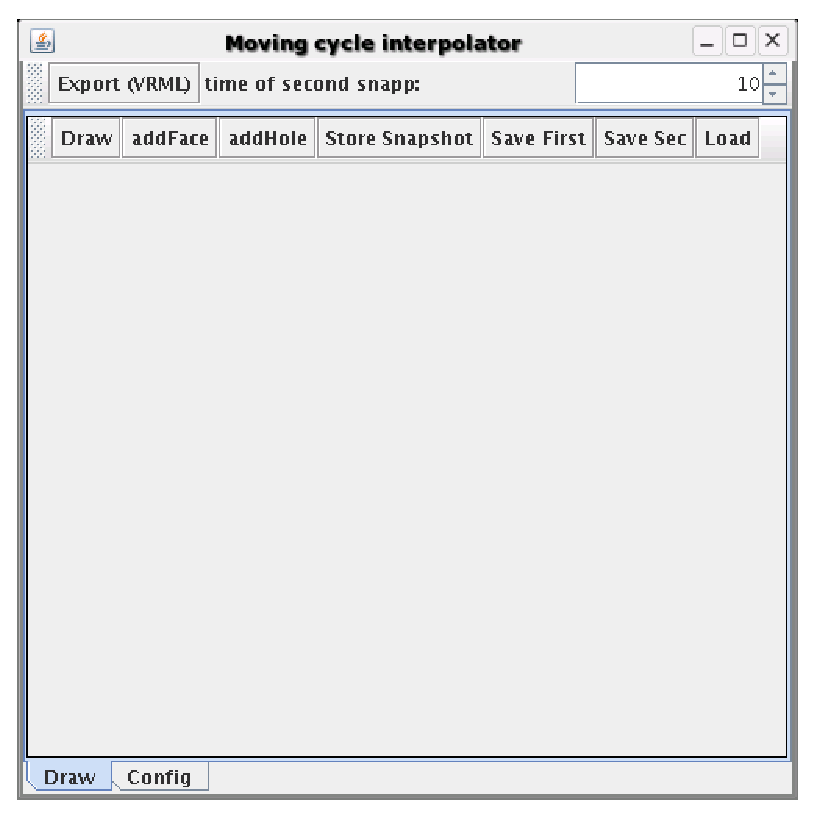
\includegraphics[scale=.8]{/home/java/Documents/Tex/Tex/start.eps}
   \caption{Der Startbildschirm}
   \label{fig:start}
\end{figure}

\section{Zeichnen einer Region}
Direkt nach dem Starten der Anwendung kann man anfangen, das erste Face zu zeichnen.  Das Zeichnen geht immer so vor sich, dass man die Punkte des Polygons nacheinander mit der Maus anklickt. Der neue Punkt und die dazugeh"orige Linie werden direkt dargestellt. 

Das Polygon muss nicht geschlossen werden, aber es ist zu beachten, dass alle Polygone einfache Polygone sein m"ussen. Eine entsprechende "Uberpr"ufung findet nicht statt.

Zum Zeichnen einer Region stehen folgende Werkzeuge bereit:
\begin{itemize}
\item Draw

Dieser Button l"oscht alle bereits eingegebenen Zeichnungen und hinterl"asst ein leeres Zeichenblatt. Auch die eventuell bereits vorhandenen Schaltfl"achen f"ur die Ergebnisansichten werden ausgeblendet.

\item addHole

Hiermit kann man dem letzten Face ein Hole hinzuf"ugen. Holes unterscheiden sich von Faces darin, dass sie nicht blau sondern rot sind. Ein Hole muss komplett innerhalb seines Faces liegen. Dies sicherzustellen ist die Aufgabe des Benutzers, eine "Uberpr"ufung findet nicht statt.

\item StoreSnapshot

Soll die Zeichnung einer Region beendet werden, so muss auf diesen Button geklickt werden. Falls es der erste Schnappschuss ist, der beendet wird, so f"arbt sich dieser blasser, und man  kann den n"achsten zeichnen. Wird aber der zweite beendet, so wird das passende Match berechnet und in den zus"atzlichen Schaltfl"achen dargestellt, die sich in ,,Die verschiedenen Ergebnisansichten`` finden.
\end{itemize} 

\section{Importieren / Exportieren}
Zum Importieren und Exportieren von Schnappsch"ussen, die mit diesem Programm erzeugt wurden, stehen drei Schaltfl"achen zur Verf"ugung:

,,Save First``, ,,Save Sec`` und ,,Load``. Wird auf einen der beiden Save-Buttons gedrückt, so "offnet sich ein Dateiauswahl-Dialog, in dem ein Dateiname f"ur die Schnappschuss-Datei angeben werde kann.

Mit Hilfe des Load-Buttons k"onnen Sie dann diese Schnappsch"usse einzeln wieder laden. Falls Sie bereits zwei Schnappsch"usse in dem Programm haben, so dr"ucken die bitte ,,Draw``, bevor Sie neue Dateien einlesen.
\section{Konfigurieren des Matchings}
Hinter der Schaltfl"ache ,,Config`` verbirgt sich ein Dialogfenster (siehe Abbildung \vref{fig:Config}), in dem einige Einstellungen vorgenommen werden k"onnen:

\begin{itemize}
\item VRML Filename und VRML Application

Erl"auterungen zu diesen Feldern befinden sich in dem Unterkapitel ,,Die verschiedenen Ergebnisansichten / VRML-Export``

\item Auswahlfeld f"ur die Art des Matchings

Hier kann man ausw"ahlen, welches Matching man gerne ausf"uhren m"ochte. Die zur Zeit verf"ugbaren Matching-Methoden werden in der Arbeit ausf"uhrlich erl"autert.

\item Schieber f"ur die Parameter der Einzelmatches

Hier kann man einigen Einzel-Matches, zur Zeit dem OverlappingMatch und den Referenzpunktverfahren, einen Parameter "ubergeben. Hierbei ist zu beachten, dass dieser Parameter je nach Art des Matches unterschiedliche Auswirkungen hat.

\item Schieber f"ur die Parameter des Optimalmatches

Das \textit{OptimalMatch} setzt sich aus den EinzelMatches zusammen, indem es verschiedene Einzelmatches mit verschiedenen Parametern ausf"uhrt und diese dann bewertet. In diese Bewertung flie"sen mehrere Kriterien gewichtet ein. Mit Hilfe dieser Schieber lassen sich die Gewichtungen der Einzel-Kriterien ver"andern.

\item Die Einzel-Bewertungen des Matches

In diesen Feldern finden Sie die Bewertungen des aktuellen Matches aufgeschl"usselt nach den einzelnen Kriterien.
\end{itemize} 
\begin{figure}
   \centering
   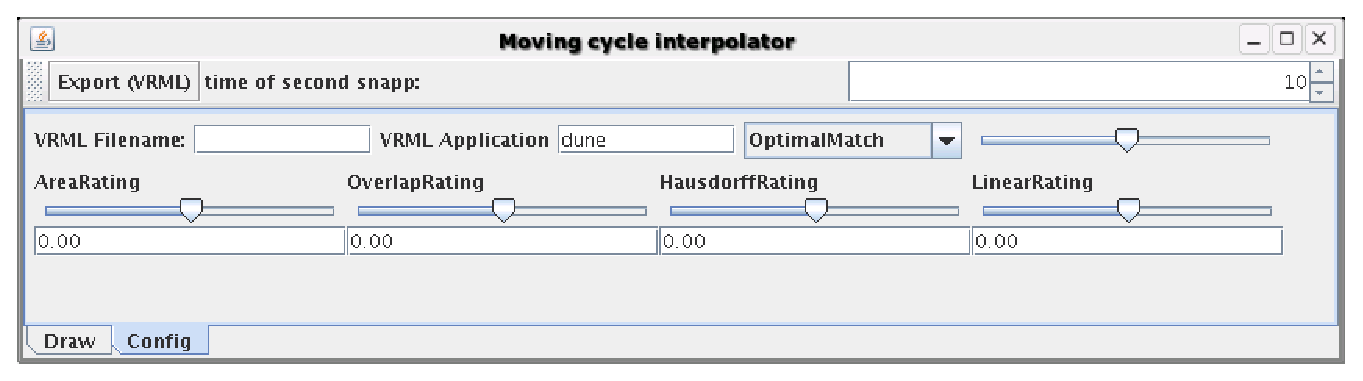
\includegraphics[scale=.65]{/home/java/Documents/Tex/Tex/Config.eps}
   \caption{Der Config-Dialog}
   \label{fig:Config}
\end{figure}
\section{Die verschiedenen Ergebnisansichten}
SoSobalder zweite ScSchnappschussbgeschlossen wird, erscheinen einige neue Schaltfl"achen, in denen Sie das Resultat des Matchings finden.

Bei den Erl"auterungen dieser Schaltfl"achen benutze ich die ScSchnappsch"ussesie in Abbildung \vref{fig:Splits} dadargestelltind.
\begin{figure}
   \centering
   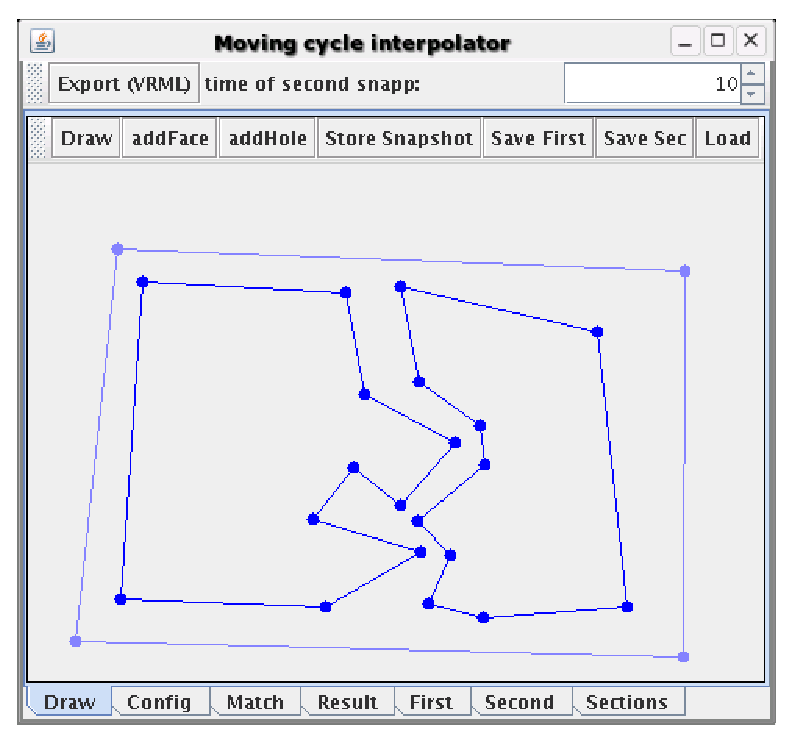
\includegraphics[scale=.8]{/home/java/Documents/Tex/Tex/Splits.eps}
   \caption{Das Beispiel}
   \label{fig:Splits}
\end{figure}
\subsection{Match}
In diesem Bildschirm (siehe Abbildung~\vref{fig:Match}) finden sich die beiden Schnappsch"usse in derselben Darstellung wie in ,,First`` und ,,Second``. In dem entsprechenden Kapitel wird diese Darstellung n"aher erl"autert. 

W"ahlt man ein Element in einer der beiden Darstellungen aus, so wird das gematchte Element der anderen Darstellung selektiert. 

In der rechten oberen Ecke des Fensters befindet sich deer Name des \textit{Matches}, eine Erl"auterung zu diesem und die Bewertung in den Kategorien. Im Falle eines \textit{OptimalMatches}, findet sich hier eine Liste mit allen Einzelmatches, die zu diesem Ergebnis kommen.
\begin{figure}
   \centering
   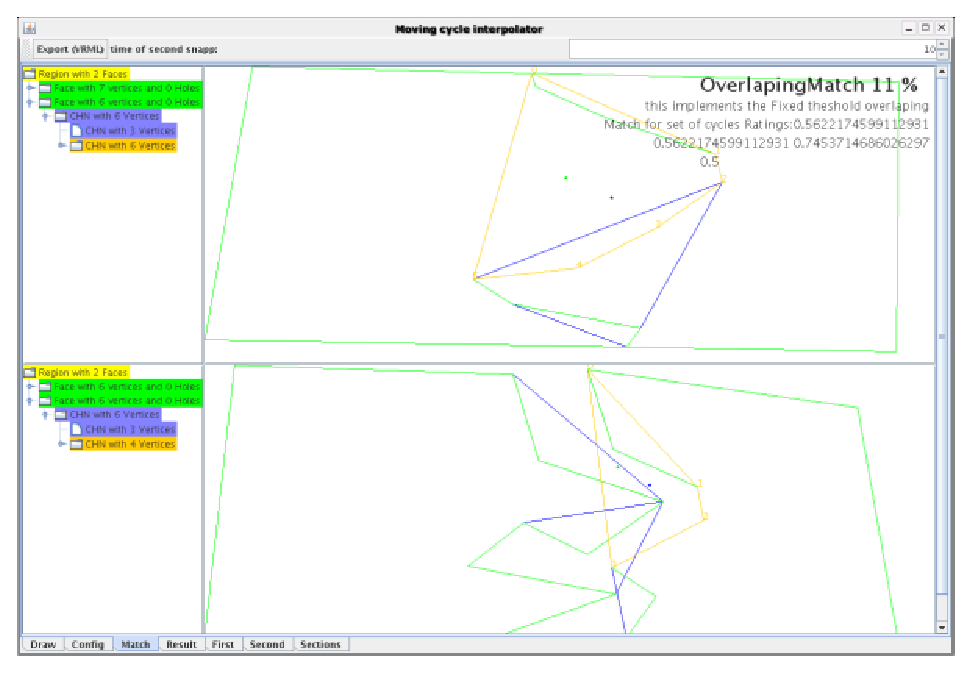
\includegraphics[scale=.8]{/home/java/Documents/Tex/Tex/Match.eps}
   \caption{Die Match-Darstellung}
   \label{fig:Match}
\end{figure}

\subsection{Result}
In diesem Bildschirm (siehe Abbildung \vref{fig:Result}) findet man eine isometrische Darstellung des Matches. Hier kann man  beide Schnappsch"usse wiederfinden. Der erste ist blau gezeichnet, der zweite rot. Die Linien, die die beiden verbinden sind grau. 

Mit Hilfe des Zeit-Einstellers in der obersten Toolbar kann den zweiten Schnappschuss weiter nach hinten rechts verschoben bzw. zur"uckgeholt werden. 

\begin{figure}
   \centering
   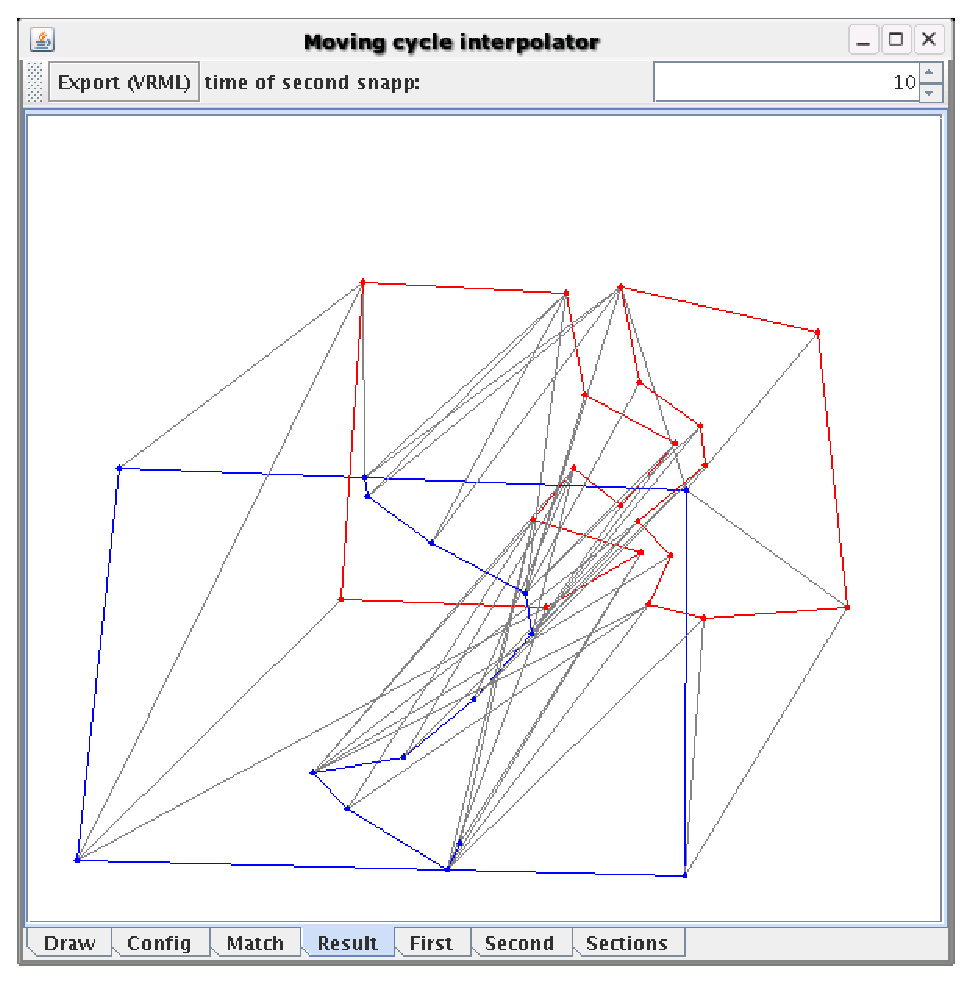
\includegraphics[scale=.6]{/home/java/Documents/Tex/Tex/Result.eps}
   \caption{Die Result-Darstellung}
   \label{fig:Result}
\end{figure}
\subsection{First und Second}
In dieser Ansicht (in Abbildung \vref{fig:Second} findet sich ,,Second`` als Beispiel) findet man zwei Darstellungen des \textit{ConvexHullTrees} eines Schnappschusses. Links finden Sie eine Baum\-ansicht des \textit{ConvexHullTrees}.

Diese Darstellung erm"oglicht es, in dem Baum zu navigieren und Elemente zu selektieren. Mehrfachselektionen kann man vornehmen, indem man beim Klicken die Strg oder die Umschaltaste h"alt. Die einzelnen Elemente des Baumes sind farblich zu unterscheiden.

Die Farben bedeuten:
\begin{itemize}
\item Gelb Region
\item Gr"un Face
\item Blau ConvexHullTreeNode
\item Rot Hole
\item Orange Selektion
\end{itemize} 

Rechts befindet sich eine Darstellung des Baumes als Menge von Polygonen. Die Farbgebung entspricht der oben genannten, daß die Region ist nicht extra dargestellt. Jedes \textit{Face} ist durch das Polygon seines \textit{Cycles} dargestellt, jedes Element eines \textit{ConvexHullTrees}, einschlie"slich der \textit{Holes}, ist durch seine konvexe H"ulle dargestellt. Selektiert man ein Element in der Baumansicht, so f"arbt sich dieses orange, die Ecken der konvexen H"ulle werden durchnummeriert und Schwerpunkt (blau) und Steiner-Punkt (gr"un) werden dargestellt.

\begin{figure}
   \centering
   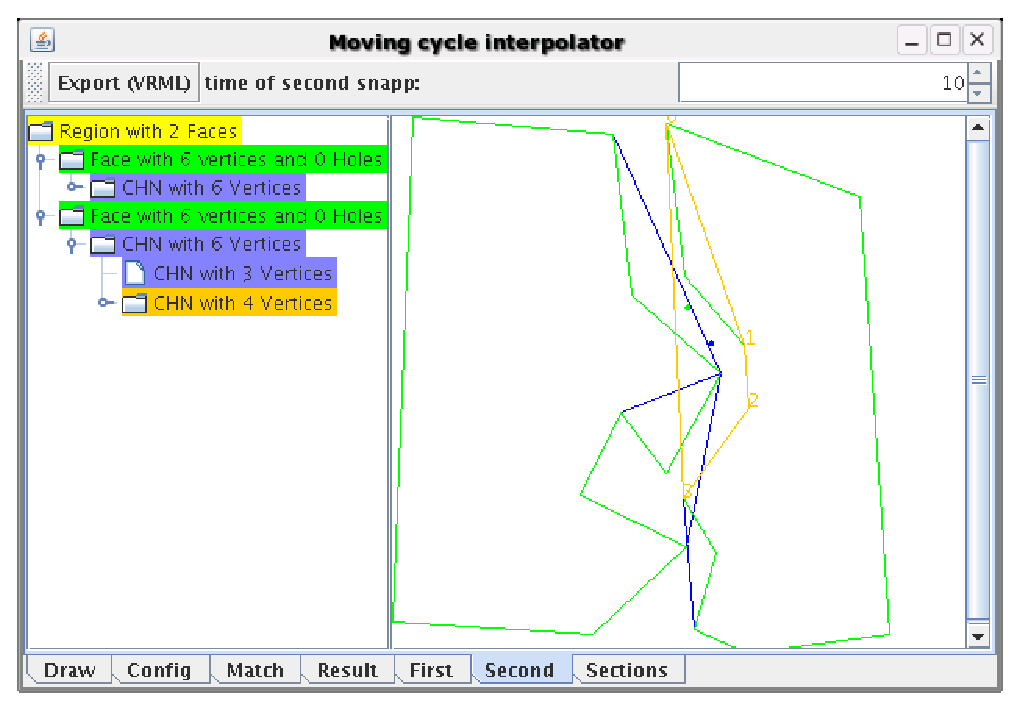
\includegraphics[scale=.8]{/home/java/Documents/Tex/Tex/Second.eps}
   \caption{Die ConvexHullTree-Darstellung des zweiten Schnappschusses}
   \label{fig:Second}
\end{figure}
\subsection{Sections}
In dieser Darstellung (Abbildung \vref{fig:Sections}) befinden  sich interpolierte Schnappsch"usse, die aus dem Match erstellt wurden. In dem Feld mittig "uber der Darstellung kann gew"ahlt werden, wieviele Schnappsch"usse betrachtet werden sollen 

Diese tauchen dann in dem Zeichenbereich dieser Seite auf. Der Erste und der Letzte entsprechen dem ersten und dem zweiten Schnappschuss, den Sie eingegeben haben.
\begin{figure}
   \centering
   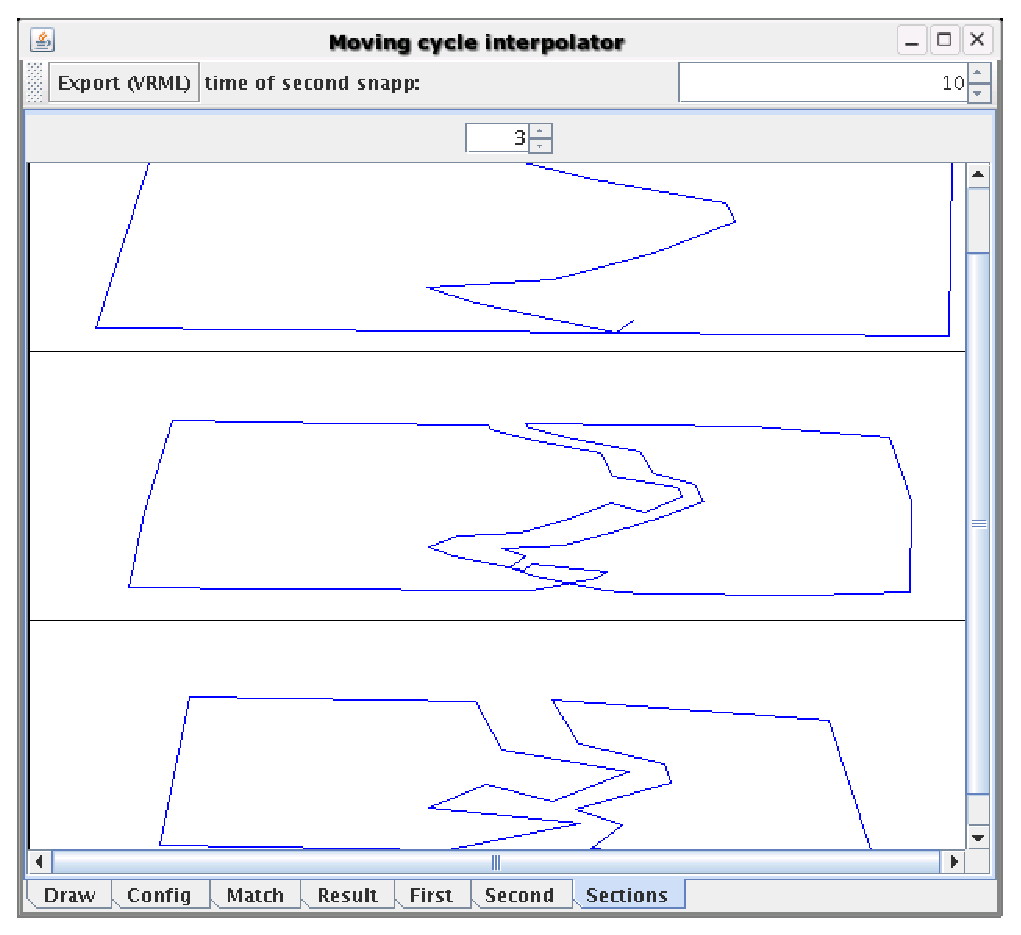
\includegraphics[scale=.8]{/home/java/Documents/Tex/Tex/Sections.eps}
   \caption{Drei Sections unseres Beispieles}
   \label{fig:Sections}
\end{figure}
\subsection{VRML-Export}
Das Tool bietet die M"oglichkeit, ein Match in eine VRML-Datei zu exportieren und so eine ansprechende 3D-Darstellung zu erhalten. Zu dem VRML-Export geh"oren vier GUI-Elemente:
\begin{itemize}
\item VRML Filename im Config-Dialog

 In diesem Feld kann man den gew"unschten Dateinamen angeben, den die neue VRML-Datei bekommen soll. Die Erweiterung .vrml wird automatisch erg"anzt
\item VRML Application im Config-Dialog

Tr"agt man in diesem Feld einen Konsolenbefehl ein, mit dem man einen VRML-Viewer startet, so startet das Tool diesen Viewer direkt nach dem Export mit der neuen Datei.

\item Der ,,Zeit-Einsteller`` in der obersten Toolbar

Mit diesem Control kann die ,,H"ohe`` der 3D-Darstellung bestimmt werden. Kleine Werte f"uhren zu flachen Polyedern, gro"se zu hohen.
\item Der ,,Export (VRML)``-Button in der obersten Toolbar

Durch den Klick auf diesen Button wird der Export ausgel"ost. Die VRML-Datei der gew"unschten H"ohe und mit dem gew"ahlten Namen wird erzeugt und direkt in dem Viewer der Wahl ge"offnet.
\begin{figure}
   \centering
   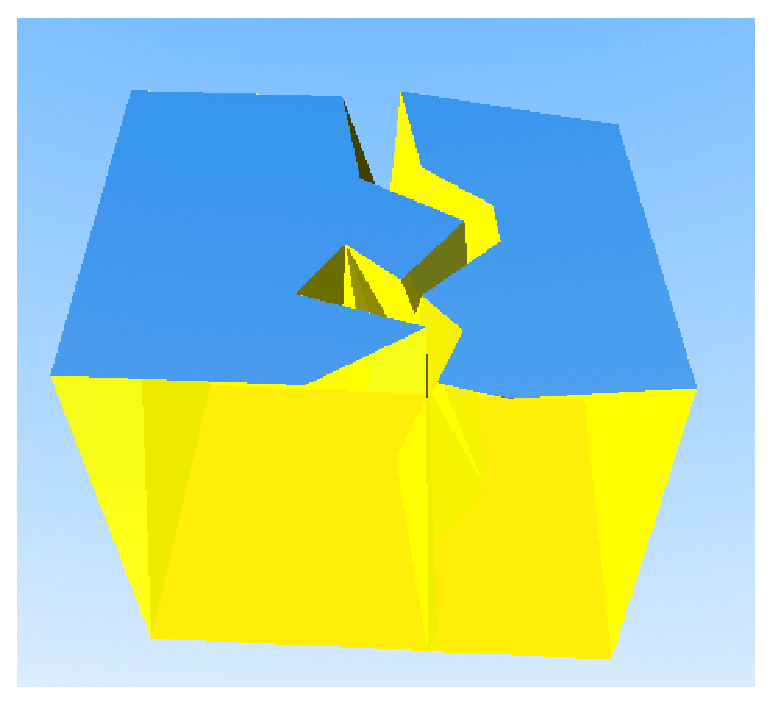
\includegraphics[scale=1]{/home/java/Documents/Tex/Tex/vrml.eps}
   \caption{Das Beispiel in einem Vrml-Viewer}
   \label{fig:vrml}
\end{figure}
\end{itemize}
